% base document setting
\documentclass[a4,paper,12pt]{article}

% load packages
\usepackage{pkg/layout_online}
\usepackage{pgfplots}
\usepackage{pgfplotstable}
\usepackage{filecontents}
\usepackage{pkg/pgf-pie}

% user defined macros

% load glossary entries
%\input{gls/glossar}	% glossary
%\input{gls/acronyms}	% actronyms
%\makeglossaries

\newcommand{\changefont}[3]{
	\fontfamily{#1} \fontseries{#2} \fontshape{#3} \selectfont
}

\newtoggle{printversion}		% definition for print or onlineversion
%\toggletrue{printversion}		% uncomment for printversion
\togglefalse{printversion}		% uncomment for onlineversion

\newtoggle{measurementdetails}		% definition for full measurement details or summary
%\toggletrue{measurementdetails}	% uncomment for full details
\togglefalse{measurementdetails}	% uncomment for summary

% document
\begin{document}
	\selectlanguage{english}
	
	% titlepages
	\thispagestyle{empty}


\begin{titlepage}

	\begin{center}
	
	% Oberer Teil der Titelseite:
	%\includegraphics[width=0.15\textwidth]{./logo}\\[1cm]    
	\textsc{
		\LARGE FH Joanneum\\~\\Graz}\\[1.5cm]
	\vfill{}
	\large Model Based Design
	\\[0.5cm]
	% Title
	\newcommand{\HRule}{\rule{\linewidth}{0.5mm}}
	\HRule
	\\[0.4cm]
	{
		%\Huge \bfseries Industrieprojekt\\
	        %~\\
	        %\large Aufbau eines 800W Phase-Shift Resonanzwandlers}\\[0.4cm]
	
		\Huge \bfseries 02 Solar Cell \\
	        ~\\
	        \large Training Unit 2 Solar Cell }
	\\[0.4cm]
	\HRule
	\\[0.5cm]
	
		%\large zur Erlangung des akademischen Grades \\
		%	Bachelor of Science in Elektrotechnik \\
		%	vorgelegt am Departement Technik \& Architektur \\
		%	der Hochschule Luzern, Schweiz CH
%		\large zur fachlichen Vertiefung im Bereich Leistungselektronik \\
%			vorgelegt am Departement Technik \& Architektur \\
%			der Hochschule Luzern, Schweiz CH
	
	\vfill{}
	
	% Author and supervisor
	\begin{minipage}{0.4\textwidth}
	    \begin{flushleft} \large
		\emph{Autor}\\
	        David B. Heer\\ ~ \\
%		\emph{Geheimhaltungsstufe} \\
%		Einsicht nach Rücksprache\\ ~ \\
%		\emph{Eingabe der Arbeit}\\
		Graz, \today
	    \end{flushleft}
	\end{minipage}
	\hfill
	\begin{minipage}{0.4\textwidth}
	    \begin{flushright} \large
	        \emph{Lecturer} \\
	        Alfred Steinhuber \\ ~ \\
%		\emph{Experte} \\
%		Prof. Dr. Adrian Omlin \\ ~ \\
%		\emph{Industriepartner} \\
%		Muster \\
	    \end{flushright}
	\end{minipage}
	
	\end{center}

\end{titlepage}

	
	
	\tableofcontents
	\clearpage
	
	%% document contents
	\part{Flight of a Model Rocket}
	%\clearpage
%\clearpage
%\input{../introduction/problem.tex}
%%\clearpage
%\input{../introduction/goal.tex}
%%\clearpage
%\input{../introduction/mission.tex}
\section{Introduction}
\todo{Grundlagen}

	\begin{enumerate}
		\item \textbf{Acceleration with constant force]} 0.15 seconds with 16N
		\item \textbf{Parabelflight} Until the parachute ist open at a velocity of $-20^m/_s$
		\item \textbf{Parachute flight} Constant velocity of $-20^m/_s$
	\end{enumerate}

	\begin{eqnarray}
		v\left( t\right)  &= v_0 + a * t\\
		s\left( t\right)  &= s_0 + v_0 * t + 0.5 * a * t^2
	\end{eqnarray}
	
	
	
	
\section{Model}


	\begin{figure}[H]
		\centering
		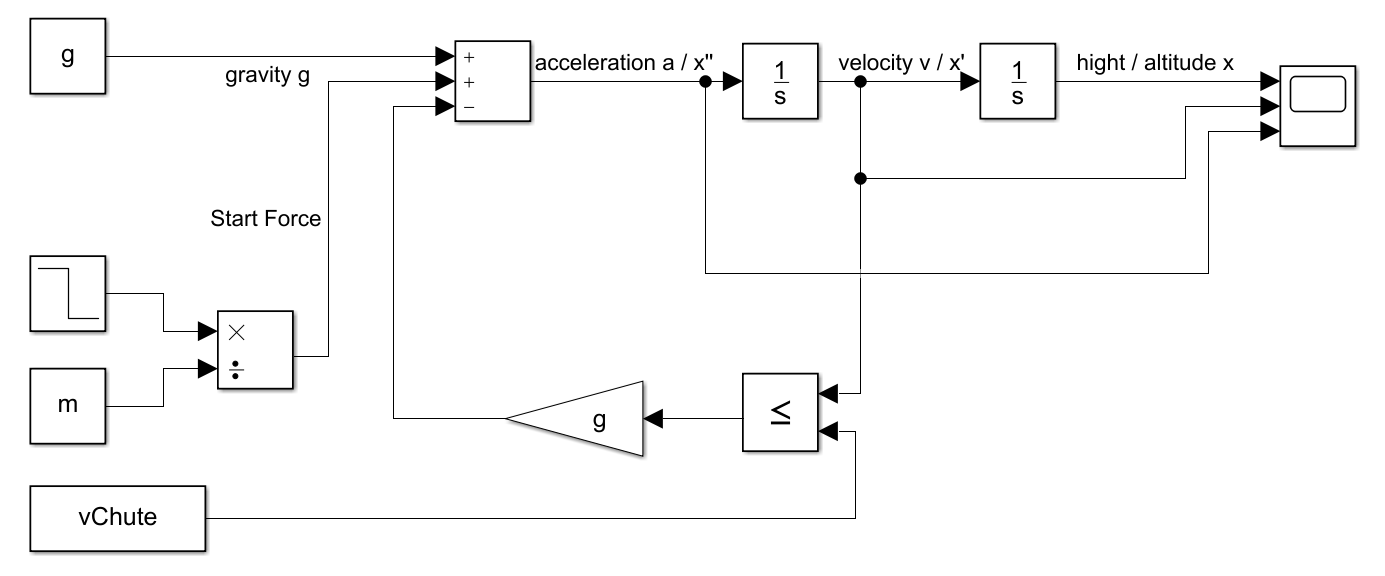
\includegraphics[width=0.7\textwidth]{figures/overview.png}
		\caption{Overview of the simulink model.}
		\label{fig:overview}
	\end{figure}


\section{Simulation}	
	
	\begin{figure}[H]
		\centering
		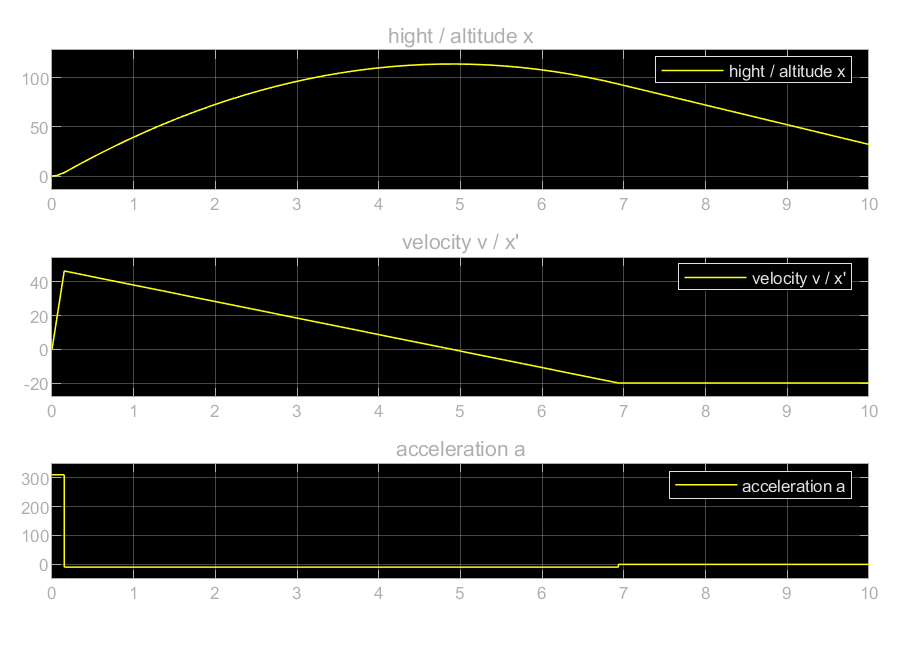
\includegraphics[width=0.7\textwidth]{figures/scope.eps}
		\caption{Scope from the Simulation.}
		\label{fig:scope1}
	\end{figure}
	
	
	
	

	\begin{lstlisting}
		clear all; clc; close all;
		
		%%
		% g inverted
		m=0.05; g=-9.81; tEngine=0.15; Force=16; vChute=-20; Dt=0.01; 
		clear t v h 
		n=1; 
		t(n)=0; v(n)=0; h(n)=0; t(2)=0;
		
		%%
		% Segment 1 
		a1=(Force-m*g)/m; 
		while (t(n) < tEngine) &&  (n < 50000) 
		n=n+1; 
		t(n)=t(n-1)+Dt; 
		v(n) =a1 *t (n) ; 
		h(n) =0.5*a1*t(n)^2;
		end;
		v1=v(n); h1=h(n); t1=t(n);
		
		% Segment 2
		while v(n)>=vChute && n<50000
		n=n+1;
		t(n)=t(n-1)+Dt;
		v(n)=v1-g*(t(n)-t1);
		h(n) =h1+v1 * (t(n)-t1 )-0.5*g* (t (n)-t1)^2;
		end
		v2=v(n); h2=h(n); t2=t(n);
		
		% Segment 3
		while h(n)>0 && n<50000
		n=n+1;
		t(n)=t(n-1)+Dt;
		v(n)=vChute;
		h (n) =h2+vChute* (t(n)-t2) ;
		end
		
		%%
		subplot(1,2,1)
		plot(t,h,t2,h2, 'ro', t1, h1, 'r+')
		xlabel('Time [s]');
		ylabel('Hight [m]');
		subplot(1,2,2)
		plot(t,v,t2,v2, 'ro', t1, v1, 'r+')
		xlabel('Time [s]');
		ylabel('Velocity [m]');
	\end{lstlisting}
	
	
	\part{Electrical System}
	\todo{input jakobs code}
	

	

	%% bibliography
	%\newpage
	%\cleardoublepage
	%\addcontentsline{toc}{section}{Literatur}
	%\bibliographystyle{ieeetr}
%\bibliographystyle{apalike}
%\bibliographystyle{alpha}

\bibliography{bib/bibliography.bib}
	%
	%
	%\addcontentsline{toc}{section}{Symbole}
	%\input{tex/symbols}
	%
	%% glossary
	%\newpage
	%\cleardoublepage
	%
	%%\clearpage
	%%\begin{multicols}{2}
	%%	\scriptsize
	%%	\glossarystyle{altlistgroup}
	%%	\glsaddall
	%	\printglossary[title=Glossar,nonumberlist]
	%	\printglossaries
	%%\end{multicols}
	%
	% list of figures
	\clearpage
	%\newpage
	%\cleardoublepage
	% \phantomsection
	\addcontentsline{toc}{section}{List of Figures}
	\listoffigures
	%
	% lsit of tables
	%\clearpage
	%\newpage
	%\cleardoublepage
	% \phantomsection
	\addcontentsline{toc}{section}{Tabellen}
	\listoftables
	%
	%	 appendix
	%	\clearpage
	%	\begin{appendices}
%\pagenumbering{roman}

%\section{Aufgabenstellung}
%\includepdf[
%	pages=1-2,
%	offset=0 -2.2cm,
%	%frame,
%	width=0.8\textwidth,
%	picturecommand={\centering},
%	pagecommand={\thispagestyle{fancy}}
%	]{../../adm/aufgabenstellung/mission.pdf}

\iftoggle{printversion}{ % content for print version --------------------------
	\addtocontents{toc}{\protect\setcounter{tocdepth}{2}}
}{ % content for online version
	\addtocontents{toc}{\protect\setcounter{tocdepth}{3}}	
}

\end{appendices}



	
\end{document}
